\documentclass{beamer-control}
\usepackage{beamer-control-singlefile}
\INCLUDEONLY{Stability}
\begin{document}
\CONCEPT{Stability}

\begin{SUMMARY}
\begin{itemize}
\item Definitions and examples
\item Stability of linear systems
\item Advanced Stability Analysis
\end{itemize}
\vfill References:
\begin{itemize}
\item \astrom{§5.3}
\end{itemize}
\end{SUMMARY}



\SUBCONCEPT{Definitions and examples}

\begin{frame}{Stability}
The stability of a dynamical system is critically important for control systems
\begin{itemize}
\item Sometimes we have an unstable system and wish to stabilise it
\item Sometimes we have a stable system and have to be careful not to destabilise it
\item We will show much later that stability and performance are inextricably linked
\begin{itemize}
\item Control loops (generally) add stability constraints to a system
\item You can design a sluggish system that will always be stable, but if you want to make it responsive you need to push against stability constraints
\end{itemize}
\end{itemize}
\end{frame}

\begin{frame}
\frametitle{Mathematical stability}
\framesubtitle{Sometimes called \emph{stability in the sense of Lyapunov}}
Define $x(t;a)$ as solution to a D.E. with initial condition $a$
\begin{itemize}
\item I.e., $x(t_0) = a$
\item We need to be specific about this because stability needs to be proven for ranges of initial condition!
\end{itemize}
Formally, stability means:
\begin{align}
\|b - a\| < \delta \;\Rightarrow\; \|x(t; b) - x(t; a)\| < \epsilon \quad \text{for all } t > 0.
\end{align}
\end{frame}

\begin{frame}
\frametitle{Example of neutral stability}
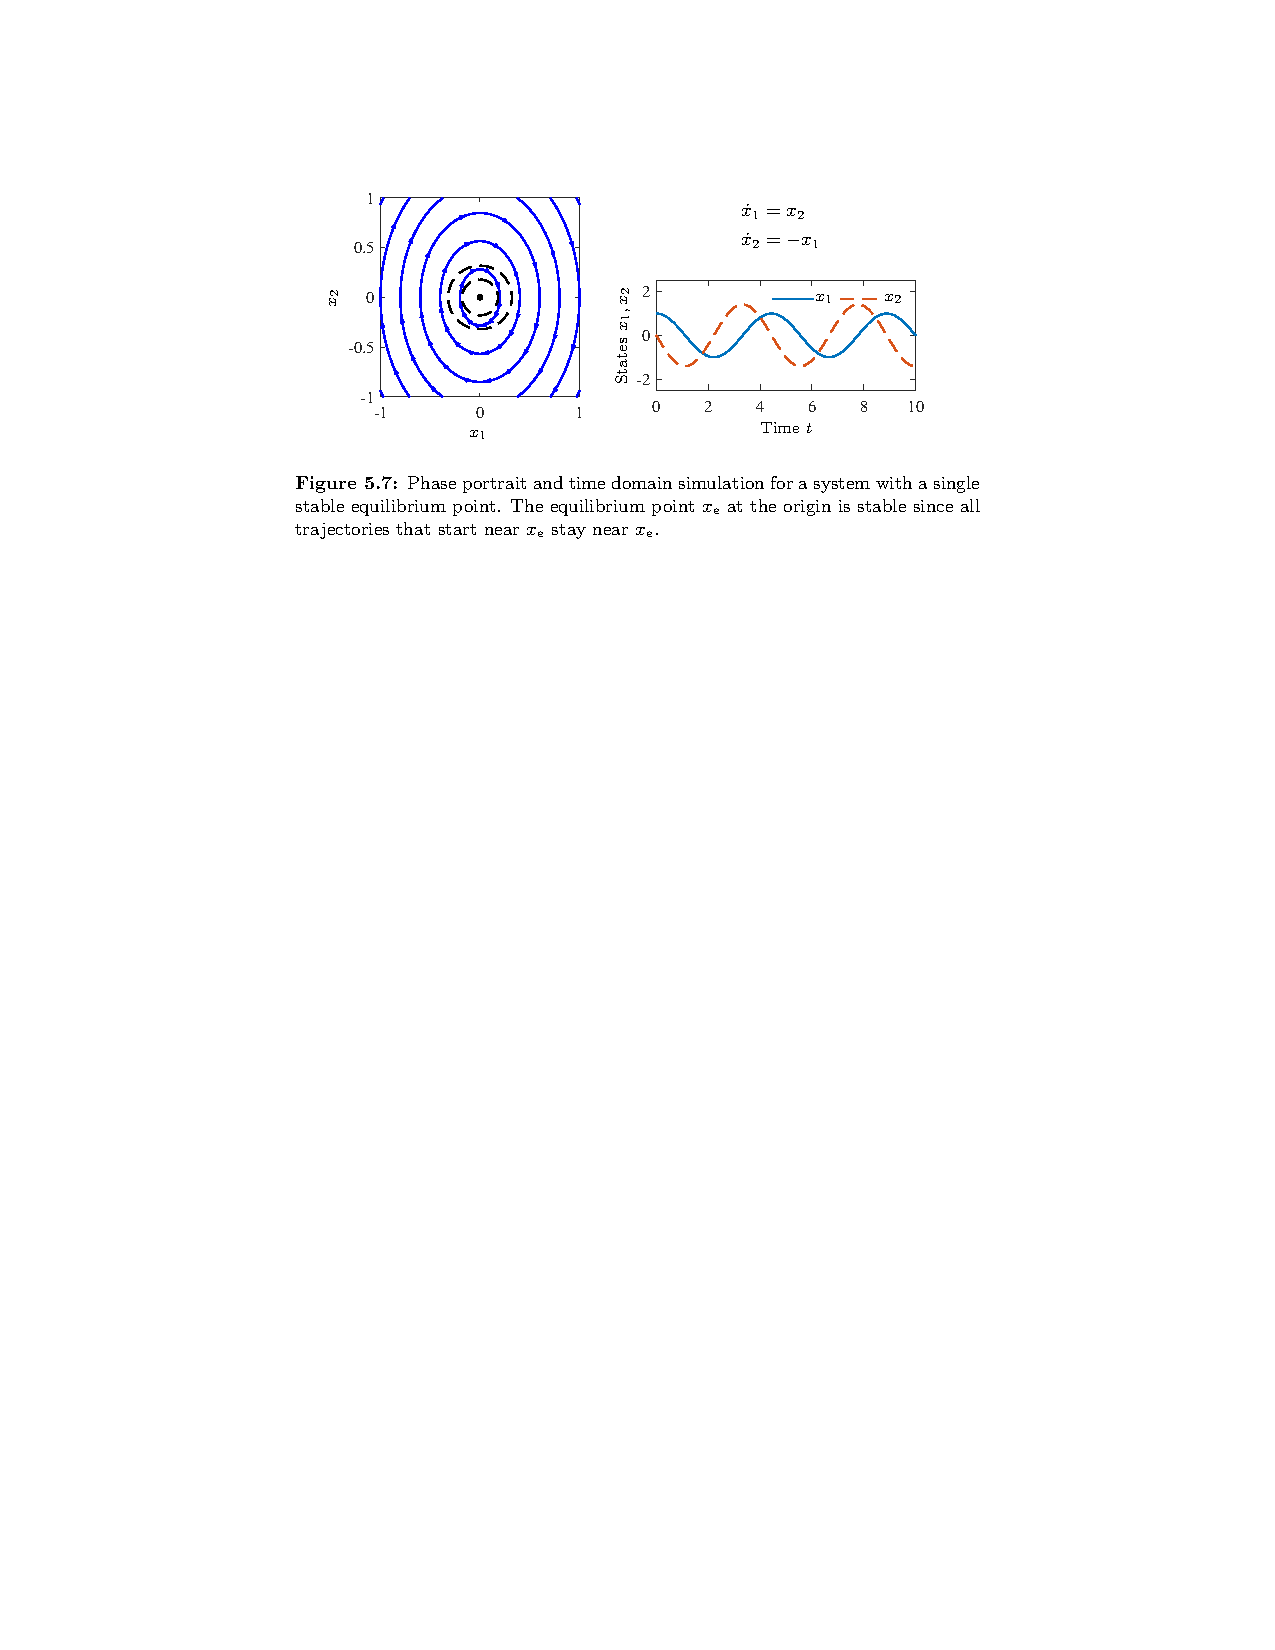
\includegraphics[width=\linewidth]{figure5.7}

\end{frame}

\begin{frame}
\frametitle{Asymptotic stability}
\begin{multline}
\|b - a\| < \delta \;\Rightarrow\; \|x(t; b) - x(t; a)\| < \epsilon \quad \text{for all } t > 0, \\
\text{\bf and} \quad \color{NorthTce} \lim_{t \to \infty} \|x(t; b) - x(t; a)\| = 0.
\end{multline}

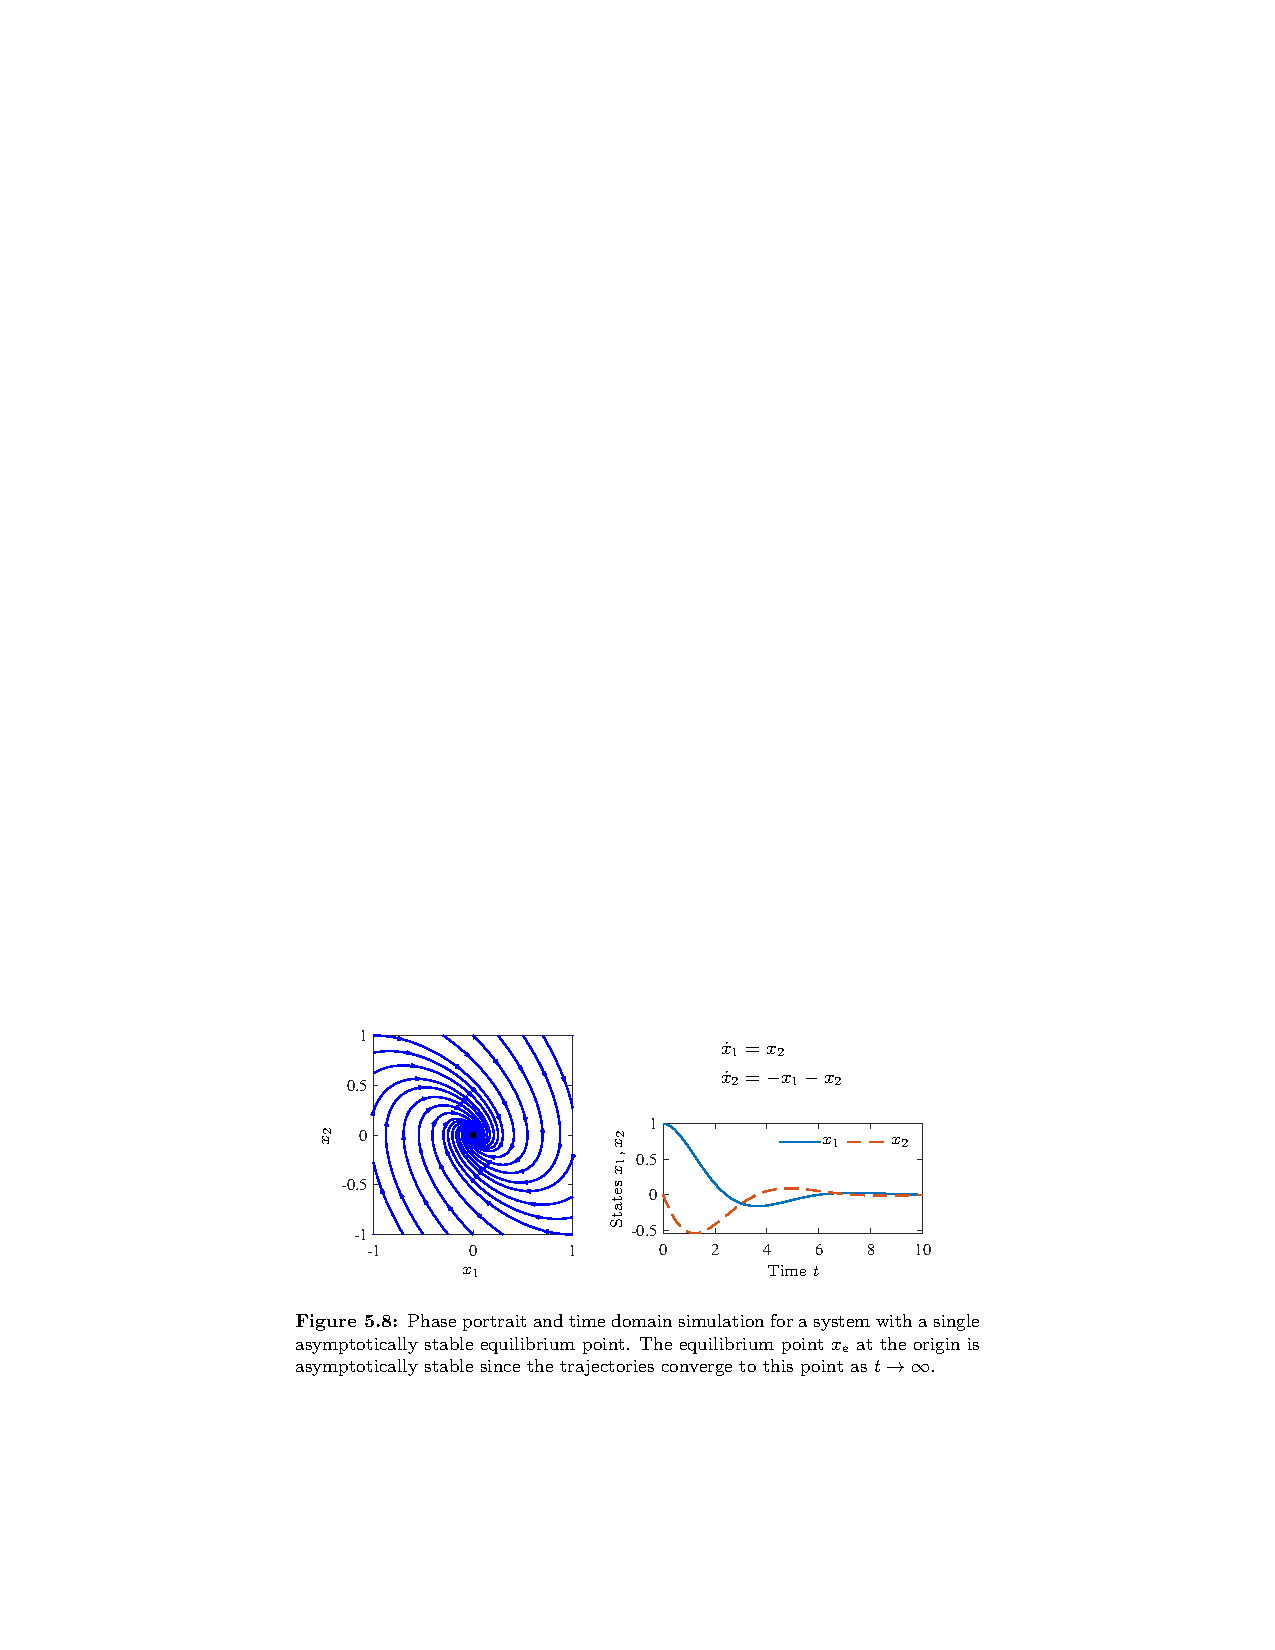
\includegraphics[width=\linewidth]{figure5.8}


\end{frame}

\begin{frame}
\frametitle{Instability}
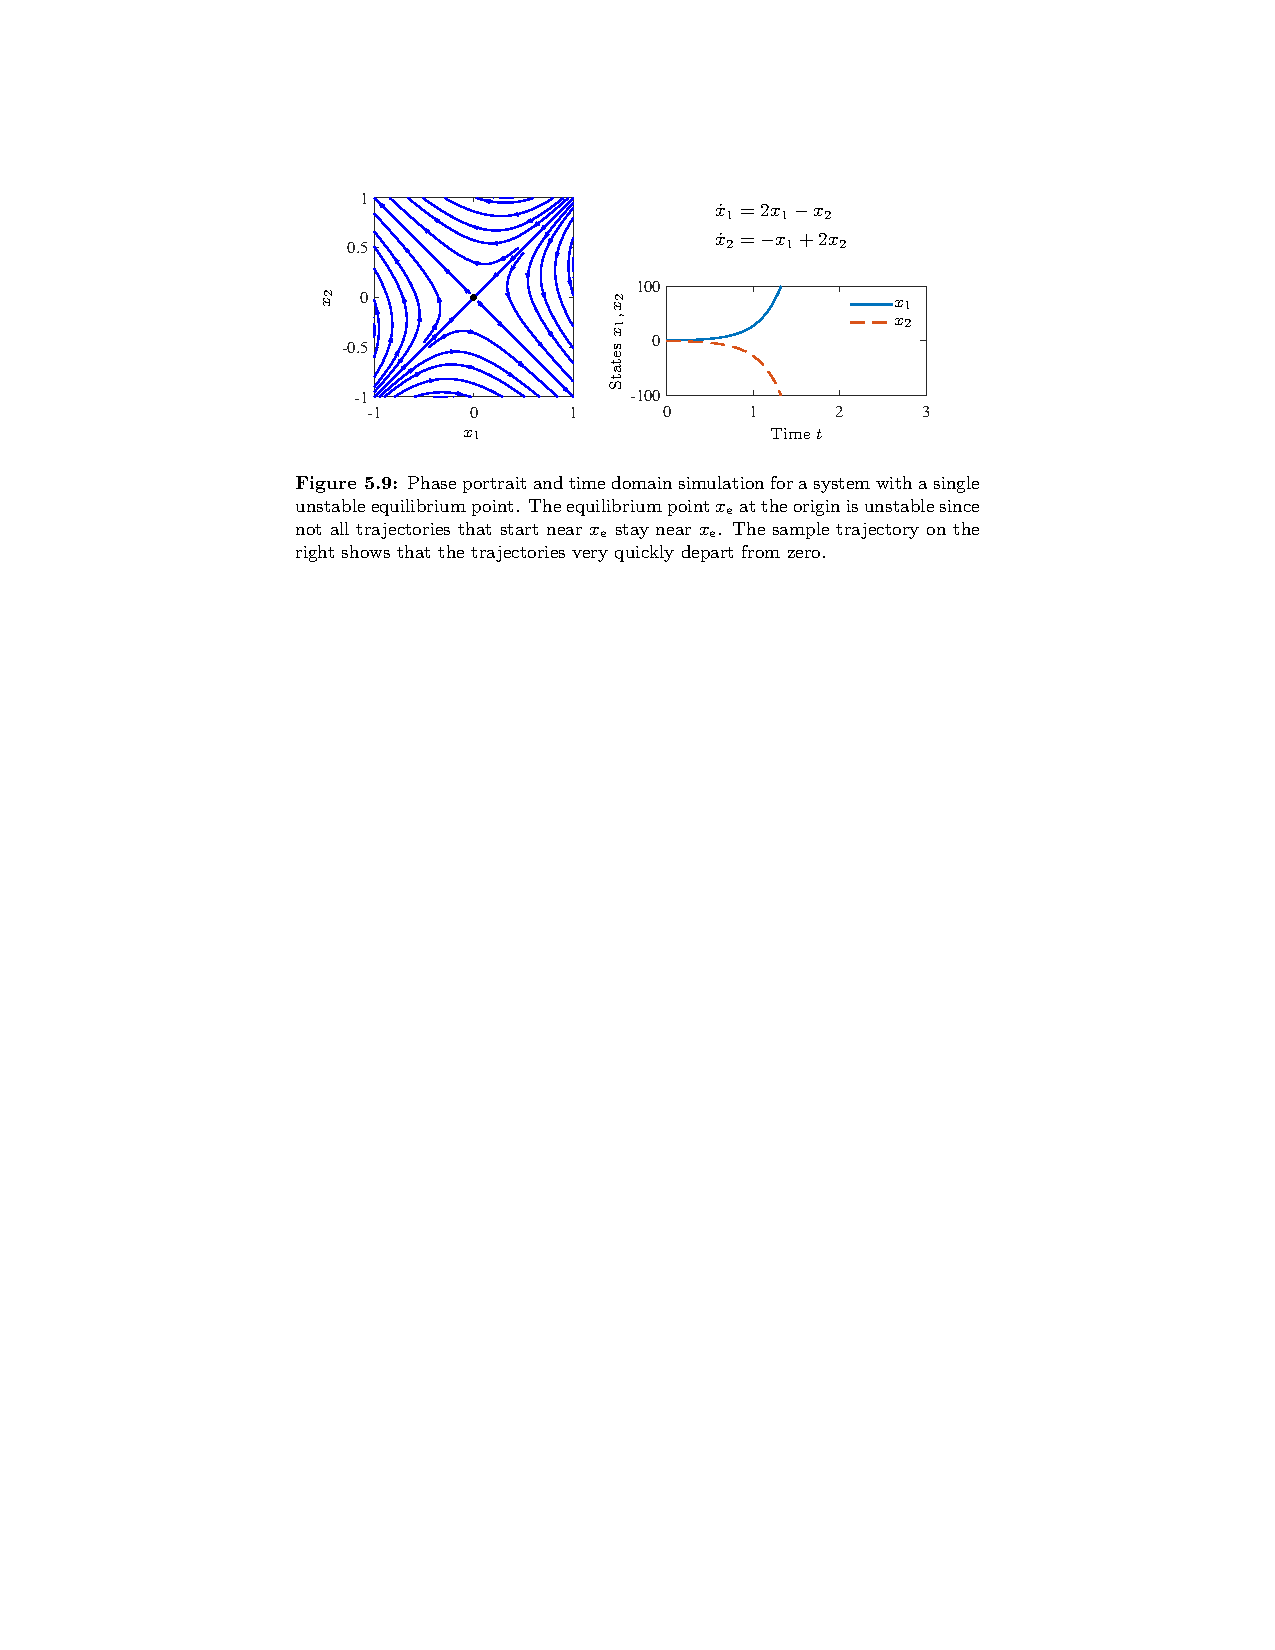
\includegraphics[width=\linewidth]{figure5.9}

\end{frame}

\begin{frame}
\frametitle{Bounded stability}
\begin{itemize}
\item For nonlinear systems, we can have stability in a local region around an equilibrium point, but not stability everywhere
\item Define a `ball' of radius $r$ around point $a$:
\begin{align}
B_r(a) = \{ x: \|x-a\| < r \}
\end{align}
\item if $x\in B_r(a)$ is stable, we have \emph{local stability}
\item For all $r>0$, we have \emph{global stability} 
\item \emph{Global asymptotic stability} is the strongest of the common classical stability notions
\end{itemize}
\end{frame}

\SUBCONCEPT{Stability of linear systems}

\begin{frame}{Stability of linear systems}{Linear systems are our key focus}
Nonlinear vs linear dynamical systems:
\begin{align}
\Deriv{x}{t} &= F(x) & \Deriv{x}{t} &= Ax
\end{align}
where $x\in \Reals^n$ and $A\in\Reals^{n\times n}$ is a square matrix

\end{frame}


\begin{frame}{Stability of linear systems}{Linear systems are our key focus}

The stability of the equilibrium point at the origin is given by 
\begin{align}
\lambda(A) \coloneq \{ s\in\mathbb{C} : \operatorname{det}(sI-A)=0 \}
\end{align}
\alert{These are the eigenvalues of the matrix $A$}
\bigskip

\begin{uncoverenv}<2->
The polynomial $\operatorname{det}(sI-A)$ is the characteristic polynomial and the eigenvalues are its roots
\end{uncoverenv}
\bigskip

\begin{uncoverenv}<3->
Eigenvalues are sometimes called `poles' and generally written, for the $j$-th eigenvalue:
\begin{align}
\lambda_j &= \sigma_j \pm \jj\ww_j
\end{align}
\end{uncoverenv}
\end{frame}

\begin{frame}
\frametitle{Stability of linear systems}
\begin{itemize}
\item Important to note: linear systems always have an equilibrium point at the origin
\item (This means that constant terms are `normalised out')
\item Because the $A$ matrix governs the entire state space, stability of linear systems implies global stability
\item Using classical ODE analytical approaches, we can see the solutions of linear systems expressed in terms of sinusoids and exponentials of their eigenvalue components:
\end{itemize}
\begin{align}
\ee^{\sigma_j t} && \sin\ww_j t && \cos\ww_j t
\end{align}
\end{frame}

\begin{frame}{Linear system stability example}{Mass-spring-damper}

\begin{align}
\dot x &= Ax + Bu & y &= Cx + Du
\end{align}
E.g., assume no input force:
\begin{align}
m\ddot q + c\dot q + kq = 0
\end{align}
\begin{align}
\dot x &= \begin{bmatrix}\dot q\\\ddot q\end{bmatrix} = \begin{bmatrix}\dot q\\- cq/m - kq/m\end{bmatrix} 
              = \begin{bmatrix}0 & 1\\- c/m & - k/m\end{bmatrix}\begin{bmatrix} q\\\dot q\end{bmatrix} = Ax
\end{align}

\end{frame}

\begin{frame}{Linear system stability example}{Mass-spring-damper}


\begin{align}
A &= \Matr{0 & 1\\- c/m & - k/m} = \Matr{0 & 1\\- \bar c & - \bar k} \\
sI-A &= \Matr{s & 0\\0 & s} - \Matr{0 & 1\\- \bar c & - \bar k} = \Matr{s & -1\\ \bar c & s+ \bar k} \\
\det(sI-A) &= (s)(s+ \bar k) - (-1)(\bar c) = s^2 + \bar k s  + \bar c
\end{align}
Therefore $\sigma_{1,2}<0$ and $\ee^{\sigma_{1,2} t}\to 0$ as $t\to\infty$: stability

\end{frame}


\SUBCONCEPT{Advanced Stability Analysis}

\begin{frame}{Stability Analysis via Linear Approximation}
\begin{align}
\Deriv{x}{t} &= \Matr{x_2\\\sin x_1-c x_2} \\
\Deriv{x}{t} &\approx \Matr{x_2\\ x_1-c x_2} = \Matr{0 & 1\\1 & -c}\Matr{x_1\\x_2} \\
\Deriv{z}{t} &= \Matr{z_2\\ -z_1-c z_2} = \Matr{0 & 1\\-1 & -c}\Matr{z_1\\z_2}
\end{align}
\end{frame}

\begin{frame}{Stability Analysis via Linear Approximation}
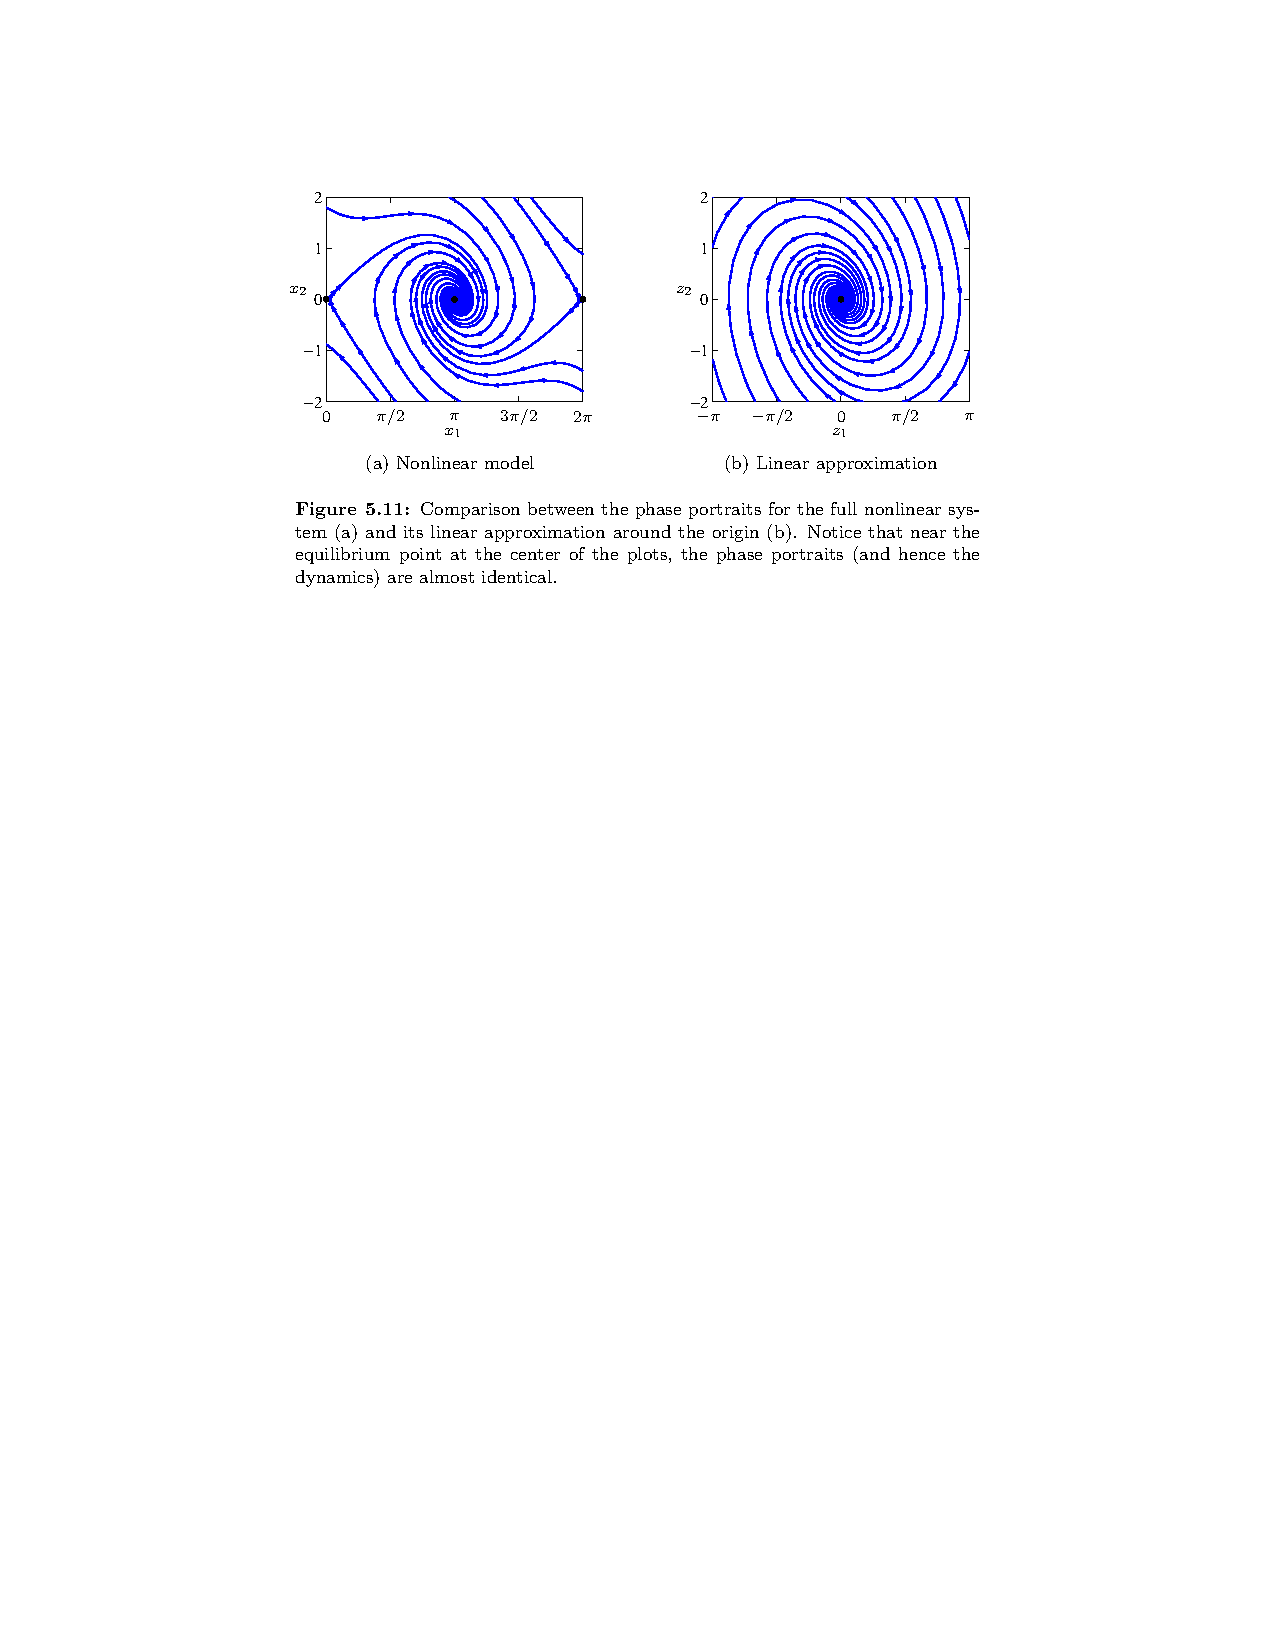
\includegraphics[width=\linewidth]{figure5.11}
\end{frame}



\begin{frame}{Stability of Limit Cycles}{This approach is quite specific --- we would typically focus on simulation models}
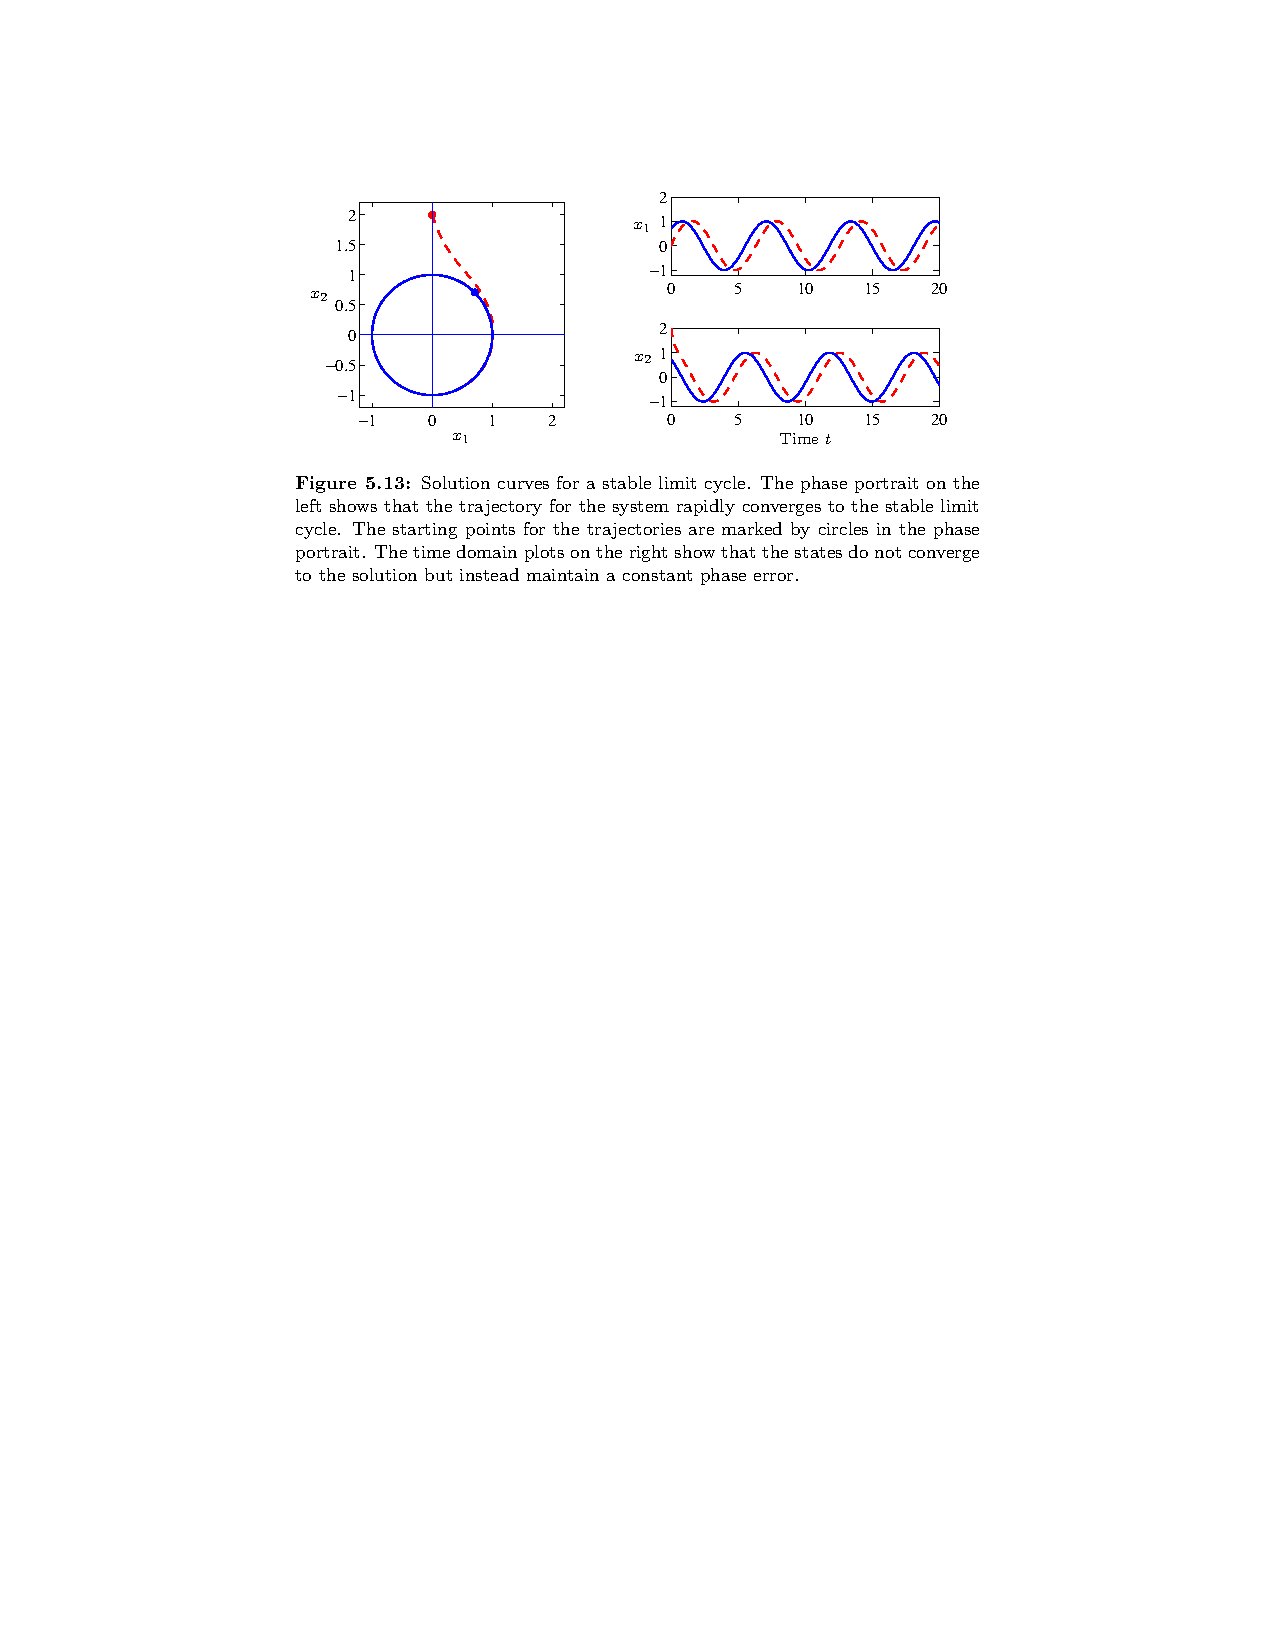
\includegraphics[width=\linewidth]{figure5.13}

\end{frame}


\begin{frame}{Lyapunov Stability Analysis — §5.4}{This section is mainly for the applied mathematicians among us}
\begin{itemize}
\item Lyapunov function $V : \Reals^n \to \Reals$ is an energy-like function to determine the stability of the system
\item In short --- if the `energy' of the system decreases to a minimum, we have found an equilibrium point
\item Lyapunov functions are not unique, but in mechanical engineering using \emph{energy} is often appropriate
\item For multi-dimensional systems, phase portraits of $V$ vs $\dot V$ can be used to illustrate complex dynamics 
\end{itemize} 
\end{frame}

\SUMMARYFRAME
\FINALE

\end{document}
